\documentclass[a4paper,11pt,reqno]{amsart}

% --------------------------------------------------------
% Packages
% --------------------------------------------------------
\usepackage[utf8]{inputenc}
\usepackage[foot]{amsaddr}
\usepackage{amsmath,amsfonts,amssymb,amsthm,mathrsfs,bm}
\usepackage[margin=0.95in]{geometry}
\usepackage{color}
\usepackage[dvipsnames]{xcolor}
\usepackage{mathtools,graphicx}
\usepackage{tcolorbox}
\usepackage{listings}
\usepackage{textcomp}
\usepackage{units}
\usepackage{hyperref}
\usepackage{ dsfont }
\usepackage{graphicx}
\usepackage{float}
\usepackage{subfig}
\usepackage{overpic}
\usepackage{tikz}

% --------------------------------------------------------
% Custom Colours
% --------------------------------------------------------
\definecolor{CommentGreen}{rgb}{0.0,0.4,0.0}
\definecolor{Background}{rgb}{0.9,1.0,0.85}
\definecolor{lrow}{rgb}{0.914,0.918,0.922}
\definecolor{drow}{rgb}{0.725,0.745,0.769}


% --------------------------------------------------------
% Typesetting Python code
% --------------------------------------------------------
\lstloadlanguages{Python}%
\lstset{
    language=Python, upquote=true, frame=single,
    basicstyle=\small\ttfamily,
    backgroundcolor=\color{yellow!30},
    keywordstyle=[1]\color{NavyBlue}\bfseries,
    keywordstyle=[2]\color{RubineRed},
    keywordstyle=[3]\color{orange!90}\bfseries,
    keywordstyle=[4]\color{Green!90}\bfseries,
    identifierstyle=,
    commentstyle=\usefont{T1}{pcr}{m}{sl}\color{MidnightBlue}\small,
    stringstyle=\color{purple},
    showstringspaces=false, tabsize=4, morekeywords={import,as},
    morekeywords=[2]{args,__init__},
    morekeywords=[3]{@property},
    morekeywords=[4]{self},
    morecomment=[l][\color{blue}]{...},
    numbers=none, firstnumber=1,
    numberstyle=\tiny\color{blue},
    stepnumber=1, xleftmargin=10pt, xrightmargin=10pt
}

\synctex=1

\hypersetup{
    unicode=false, pdftoolbar=true, 
    pdfmenubar=true, pdffitwindow=false, pdfstartview={FitH}, 
    pdftitle={ELE8088 Coursework}, pdfauthor={A. Author},
    pdfsubject={ELE8088 coursework}, pdfcreator={A. Author},
    pdfproducer={ELE8088}, pdfnewwindow=true,
    colorlinks=true, linkcolor=red,
    citecolor=blue, filecolor=magenta, urlcolor=cyan
}

% --------------------------------------------------------
% CUSTOM COMMANDS
% --------------------------------------------------------
\newcommand{\iu}{{\mathrm{i}\mkern1mu}}
\newcommand{\R}{{\rm I\!R}}
\newcommand{\N}{{\rm I\!N}}
\newcommand{\E}{{\rm I\!E}}
\newcommand{\C}{\mathbb{C}}
\newcommand{\dd}{\mathrm{d}}
\newcommand{\tran}{\intercal}
\DeclareMathOperator{\Var}{Var}
\DeclareMathOperator*{\argmin}{arg\,min}
\DeclareMathOperator*{\argmax}{arg\,max}
\DeclareMathOperator*{\minimise}{minimise}
\newcommand{\smallmat}[1]{\left[ \begin{smallmatrix}#1 \end{smallmatrix} \right]}
\newcommand{\smallplus}{{\scriptscriptstyle +}}
\newcommand{\Spp}{\mathbb{S}_{\smallplus\smallplus}}
\newcommand{\Sp}{\mathbb{S}_{\smallplus}}
\newcommand{\prob}{\mathrm{P}}

% --------------------------------------------------------
% Opening: Title and Author Names
%          Modify this section
% --------------------------------------------------------

\title[ELE8088 Coursework]{Control \& Estimation Theory}

\author[S. Chen]{ShihaoChen}

\address[Shihao Chen]{Email addresses: \href{schen45@qub.ac.uk}%
{schen45@qub.ac.uk} }
\thanks{Thanks Dr. Pantelis Sopasakis.  Version 0.0.1. Last updated:~\today.}



% --------------------------------------------------------
% Beginning of your document
% --------------------------------------------------------
\begin{document}

\maketitle



% --------------------------------------------------------
% Problem 1
% --------------------------------------------------------
\Large
\section{Problem 1}
Consider the discrete-time linear dynamical system $x_{t+1} = \gamma Ax_t + Bu_t$, where $\gamma \neq0$.
Suppose that the pair (A, B) is controllable.Show that ($\gamma$A, B) is controllable.Be careful: this exercise says
“controllable,” not “reachable.” Do not use the controllability matrix.

\textbf{Solotion:}

The controllability matrix is $C_n = [A^{n-1}B \hspace{0.5em} A^{n-2}B \hspace{0.5em} \cdots \hspace{0.5em} B ]$.

For the pair (A,B) is controllable we can steer its state to the origin from any initial state x in n steps:
$\phi(n;x;u_n) = 0$,must be solvable for $u_n$ for any $x\in\R^n$.

Which means 
\begin{equation}
    A^nx+C_nu_n = 0 \Leftrightarrow C_nu_n = -A^nx
\end{equation}
This is true iff $rangeC_n = rangeA^n$.Thus $rangeC_n = rangeA^n = range\gamma A^n$

So for the pair ($\gamma$A, B) is controllable due to 
\begin{equation}
    C_nu_n = -\gamma A^nx \Leftrightarrow \gamma A^nx+C_nu_n = 0
\end{equation}

% --------------------------------------------------------
% Problem 2
% --------------------------------------------------------

\section{Problem 2}
\subsection{}
In Handout 1, Section 1.1.6, we stated that “Lyapunov stability does not imply attractivity” and
that “Attractivity does not imply Lyapunov stability.” Demonstrate this with a couple of examples.

\textbf{Solotion:}

$\rhd$ First example for $Lyapunov \hspace{0.25em} stability \nRightarrow Attractivity$:
\begin{equation}
    x_{t+1} = x_t
    \label{3}
\end{equation}

This system is Lyapunov stable since Equation\eqref{3} over a positive invariant set $X$
is a constant function for every $\epsilon > 0$ there is a $\delta > 0$.Such that
\begin{equation}
    x_0 \in X \cap \mathcal{B_\delta} \Longrightarrow \phi(t;x_0) \in \mathcal{B_\epsilon},{\forall} t \in \mathds{N}. 
\end{equation}

But it is not globally attractive since as $t \rightarrow \infty,\phi(t;x_0) \nrightarrow 0$.

$\rhd$ Second example for $Attractivity \nRightarrow Lyapunov \hspace{0.25em} stability$:
\begin{equation}
    x_{t+1}=\left\{
    \begin{aligned}
    -2x_t, \hspace{3em} if \hspace{0.25em} |x_t| < 1 \\
    0, \hspace{3em} otherwise
    \label{5}
    \end{aligned}
    \right.
\end{equation}

For all $x_0 \in$ (-1,1) with $x_0 \neq 0$,the trajectory $x_t$ will exist (-1,1) in finite time
and $x_t \rightarrow 0$ as $t \rightarrow \infty$.Thus this system \eqref{5} is globally attractive.

But the origin is not stable since the trajectories will not stay close to zero.
\subsection{}
Consider a dynamical system $x_{t+1} = f(x_t)$ with $f(0) = 0$ and a positive invariant set X $\subseteq \R^n$.
Is it possible that the origin is $GAS$ over $X$, but not $LAS$? Justify your answer.

\textbf{Solotion:}

% If this system is $GAS$ which implies it is both Lyapunov stable and globally attractive over the 
% positive invariant set $X \subseteq \R^n$

For the system \eqref{6} over a positive invariant set $X = [0,\infty]$,the origin is $GAS$ over $X$ since 
it is both Lyapunov stable,globally attractive and $x_t$ approaches 0 much closely
and converges wherever it starts from on the right of set $X$,for the left of set $X$ it does not converge.
\begin{equation}
    x_{t+1}=\left\{
    \begin{aligned}
    0.5x_t, \hspace{3em} if \hspace{0.25em} x_t \geq 0 \\
    2x_t, \hspace{3em} if \hspace{0.25em} x_t < 0
    \label{6}
    \end{aligned}
    \right.
\end{equation}

But it is not locally sttractive over $X$ since it is not for all $x_0 \in X \cap \mathcal{B_\eta}$
there is $\eta > 0$ such that $\phi(t;x_0) \rightarrow 0$ as $t \rightarrow \infty$.

Thus it is not $LAS$.

% --------------------------------------------------------
% Problem 3
% --------------------------------------------------------

\section{Problem 3}
(This is from Handout 1) Find a $GES$ linear system, $x_{t+1} = Ax_t$,with $x_t\in\R^2$ such that the Euclidean
unit ball,$\mathcal{B} = \{x\in\R^2:\Vert x \Vert \leq 1\}$, is not an invariant set.

\textbf{Solotion:}
The Python code: \href{https://github.com/Chanawesome/ELE8088-EXTRA/blob/main/Problem3.py}{Please Click Here}.

The unit ball is not invariant for the system \eqref{7} starts from $x_0 \in \mathcal{B}$ since
there is a point $(x_2)$ in the unit ball such that $\begin{bmatrix}0.2 & -0.5 \\ 0.4 & 1.5 \end{bmatrix} x_2 \hspace{0.3em} (x_3)$ 
is not in the unit ball as shown in Fig. \ref{f3}.
\begin{equation}
    x_{t+1} = \begin{bmatrix} 0.2 & -0.5 \\ 0.4 & 1.5 \end{bmatrix} x_t
    \label{7}
\end{equation}

\begin{figure}[H]
    \centering
    % 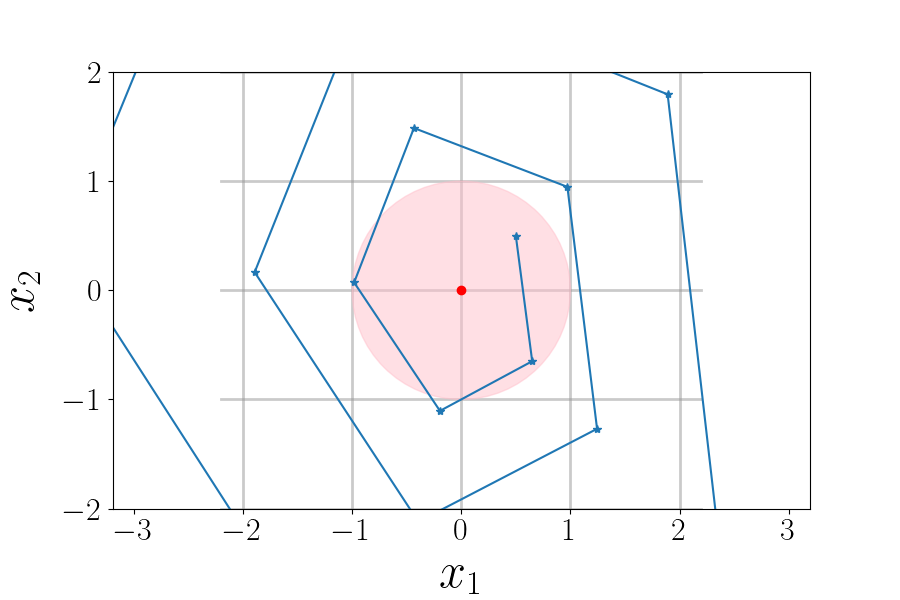
\includegraphics[height=12cm,width=14cm]{Problem3.png}
    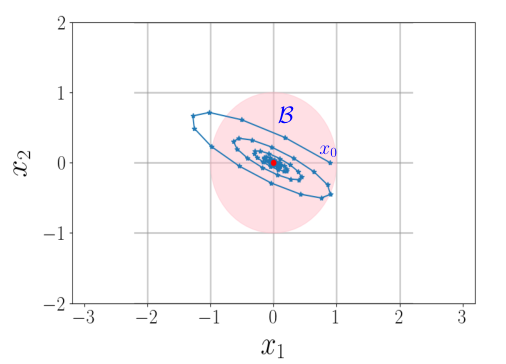
\includegraphics[width=1\textwidth]{Problem3.2.png}
    \caption{Not an invariant set}
    \label{f3}
    \end{figure}

% \begin{overpic}[height=12cm,width=1\textwidth]{Problem33.png}
%     \put(60,40){\LARGE\bfseries\color{blue}{$x_0$}}  
%     \put(52,46){\huge\bfseries\color{blue}{$\mathcal{B}$}}  
% \end{overpic}

% --------------------------------------------------------
% Problem 4
% --------------------------------------------------------
\section{Problem 4}
\subsection{}
Check whether the origin is globally exponentially stable (GES) for the discrete-time linear
dynamical system
\begin{equation}
    x_{t+1} = \begin{bmatrix} 0.9 & 0.1 & 0 \\ -0.1 & 0.9 & 0 \\ 0 & 0 & -0.3\end{bmatrix} x_t
    \label{8}
\end{equation}
using \textbf{Theorem 1.1:(Stability of Linear Systems)}:the origin is $GES$ for the linear system
$x_{t+1} = Ax_t$ over ($\R^n$) iff all the eigenvalues of $A$ are within the unit circle
(otherwise it is not attractive).

\textbf{Solotion:}

$A = \begin{bmatrix} 0.9 & 0.1 & 0 \\ -0.1 & 0.9 & 0 \\ 0 & 0 & -0.3\end{bmatrix}$
% \hspace{0.8em}
% $|\lambda I-A| = \begin{bmatrix} \lambda-0.9 & 0.1 & 0 \\ -0.1 & \lambda-0.9 & 0 \\ 0 & 0 & \lambda+0.3\end{bmatrix}=0$

Thus $\lambda_1=0.9+0.1i,\lambda_2=0.9-0.1i,\lambda_3=-0.3$.

Their modulus for $\lambda_1,\lambda_2,\lambda_3$ are $0.9055,0.9055,0.3$ respectively and they are
all less than $1$ so that this system \ref{8} is $GES$.
\subsection{}
If it is GES, determine a Lyapunov function.

\textbf{Solotion:}

The linear system $x_{t+1} = Ax_t$ is $GES$ iff given $Q \in \mathbb{S}^n_{++}$ there exists a
$P \in \mathbb{S}^n_{++}$ that satisfies the Lyapunov equation
\begin{equation}
    A^{\tran}PA-P = -Q
    \label{9}
\end{equation}
The $P$ that solves this equation is unique in $\mathbb{S}^n_{++}$ and $V(x)=x^{\tran}Px$ satisfies the
conditions of Lyapunov's theorem.

For this linear system \ref{8}.
% \begin{equation}
%     x_{t+1} = \begin{bmatrix} 0.5 & 0.3 \\ -0.7 & -0.9 \end{bmatrix} x_t
%     \label{10}
% \end{equation}

Using $Q = I = \begin{bmatrix} 1 & 0 & 0 \\ 0 & 1 & 0 \\ 0 & 0 & 1 \end{bmatrix}$ 
that the following matrix is the unique solution of the Lyapunov equation:
$P = \begin{bmatrix} 5.55556 & 0 & 0 \\ 0 & 5.55556 & 0 \\ 0 & 0 & 1.0989 \end{bmatrix}$

So $V(x) = x^{\tran}Px = x^{\tran}\begin{bmatrix} 5.55556 & 0 & 0 \\ 0 & 5.55556 & 0 \\ 0 & 0 & 1.0989 \end{bmatrix}x$.

\subsection{}
Determine an invariant set for this system that is contained in the Euclidean unit ball,
$\mathcal{B} = \{x \in \R^3:\|x\| \leq 1\}$.

\textbf{Solotion:}

For origin of the linear system \ref{8} is $GES$,the Lyapunov function \ref{9} satisfies the following bounds:
\begin{equation}
    \lambda_{min}(P)\|x\|^2 \leq V(x) \leq \lambda_{max}(P)\|x\|^2
\end{equation}
which is
\begin{equation}
    0.3\|x\|^2 \leq V(x) \leq 0.9055\|x\|^2
\end{equation}
Since $V(x)$ satisfies LDC.For $V:X\rightarrow[0,\infty]$.Then $Y={x\in X:V(x)\leq 0.9055}$
is a invariant for this system \ref{8}. 
% --------------------------------------------------------
% Problem 5
% --------------------------------------------------------
\section{Problem 5}
Consider the following discrete-time linear dynamical system
\begin{equation}
    \begin{bmatrix} a_{t+1} \\ b_{t+1} \end{bmatrix} = 
    \begin{bmatrix} \frac{1}{5}a_t+cos(b_t)-1 \\ \frac{1}{2}e^{a_t}b_t \end{bmatrix} 
    \label{12}
\end{equation}
The state of the system is the vector $x_t = [a_t \hspace{0.25em} b_t]^{\tran} \in \R^2$.
\subsection{}
Show that the origin is an equilibrium point of this dynamical system.

\textbf{Solotion:}

With $x_0 = [0 \hspace{0.25em} 0]^{\tran}$ that $ \begin{bmatrix} a_{1} \\ b_{1} \end{bmatrix} = x_1
 = \begin{bmatrix} \frac{1}{5}0+cos(0)-1 \\ \frac{1}{2}e^{0}0 \end{bmatrix} =  \begin{bmatrix} 0 \\ 0 \end{bmatrix}$.

Thus the origin is an equilibrium point of this dynamical system since $[0 \hspace{0.25em} 0]^{\tran} = f([0 \hspace{0.25em} 0]^{\tran})$.

\subsection{}
Use Theorem 2.6 (in Handout 2) to tell whether the system is locally exponentially stable.

\textbf{Solotion:}

The system state is $x_t = (a_t,b_t)$.The Jacobian is
\begin{equation}
    Jf(x) = \begin{bmatrix} \frac{1}{5} & -\sin(b) \\ \frac{1}{2}e^{a}b & \frac{1}{2}e^{a} \end{bmatrix}
\end{equation}
So  
\begin{equation}
    A = Jf(0) = \begin{bmatrix} \frac{1}{5} & 0 \\ 0 & \frac{1}{2} \end{bmatrix}
\end{equation}
The eigenvalues of A are $\frac{1}{5}$ and $\frac{1}{2}$,so $\rho(A) = \frac{1}{2} < 1$,
therefore, the origin is $LES$ for the system \ref{12}.

\subsection{}
Use Python to simulate this system starting from various initial states close to the origin. Include
a plot of the system trajectories in your report.

\textbf{Solotion:}
The Python code: \href{https://github.com/Chanawesome/ELE8088-EXTRA/blob/main/Problem5.3.py}{Please Click Here}.

\begin{figure}[H]
    \centering
    % 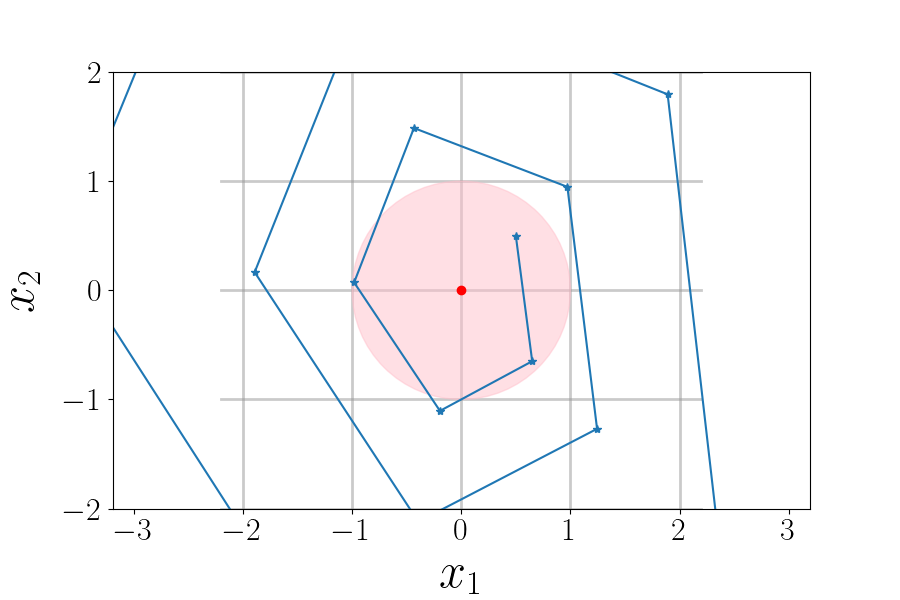
\includegraphics[height=12cm,width=14cm]{Problem3.png}
    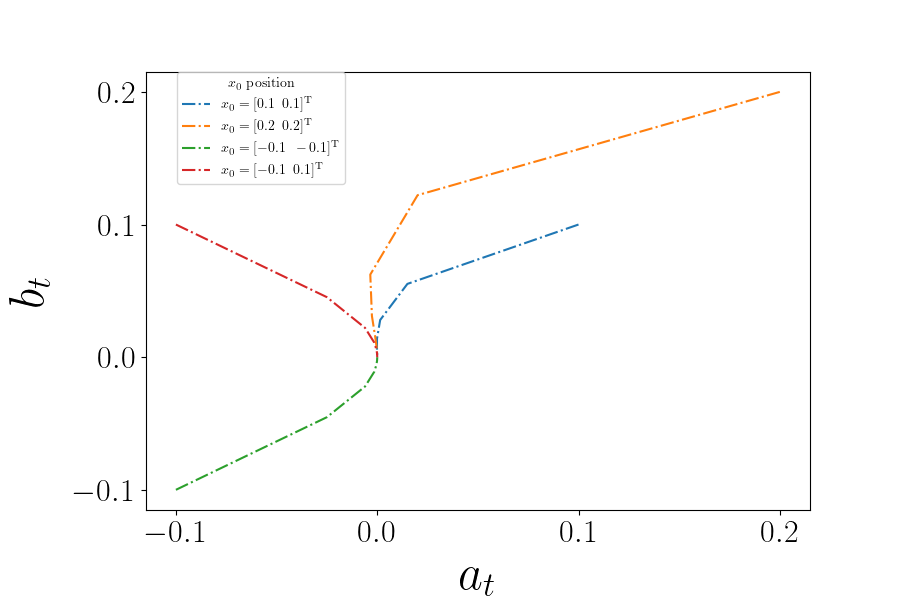
\includegraphics[width=1\textwidth]{Problem5.3.png}
    \caption{Simulation from various initial states}
    \label{f5}
    \end{figure}

% --------------------------------------------------------
% Problem 6
% --------------------------------------------------------
\section{Problem 6}
\subsection{}
Prove that the function $f:(0,\infty) \rightarrow \R $ with $f(x) = x^2+x-2022 \log x$ is convex.

\textbf{Solotion:}

% Define $\lambda \in [0,1]$ and $x_1,x_2 \in (0,\infty)$,
% \begin{subequations}
%     \begin{align}
%         f(\lambda x_1+(1+\lambda)x_2) = (\lambda x_1+(1+\lambda)x_2)^2+(\lambda x_1+(1+\lambda)x_2)
%         \\
%         -2022\log(\lambda x_1+(1+\lambda)x_2) \notag
%         \\ 
%         =\lambda^2(x_1+x_2)^2+\lambda(2x_2^2+2x_1x_2+x_1+x_2)+x_2^2+x_2
%         \\
%         -2022\log(\lambda x_1+\lambda x_2+x_2) \notag 
%     \end{align}
% \end{subequations}
% And
% \begin{subequations}
%     \begin{align}
%         \lambda f(x_1)+(1-\lambda)f(x_2) = \lambda(x_1^2+x_1-2022 \log x_1)
%         \\
%         +(1-\lambda)(x_2^2+x_2-2022 \log x_2) \notag
%         \\
%         =\lambda2022\log \frac{x_2}{x_1}-2022\log x_2+\lambda(x_1^2-x_2^2+x_1-x_2)+x_2^2
%     \end{align}
% \end{subequations}

The gradient for this function is $\triangledown f(x) = 2x+1-2022\frac{1}{x\ln 10}$ and 
its Hessian is $\triangledown^2f(x) = 2+2022\frac{\ln10+\frac{x}{10}}{x^2\ln^{2}10}$.

Since $x\in(0,\infty)$ that $\ln10+\frac{x}{10}$ and $x^2\ln^{2}10$ are both greater than 0,thus
$\triangledown^2f(x) > 0$,so this function is convex.

\subsection{}
Use Python to solve the minimisation problem 
\begin{equation}
\minimise_{\substack{1\leq x \leq 100}}x^2+x-2022 \log x,
\label{17}
\end{equation}
that is, determine a minimiser and the optimal value of this problem. Include a link to your code and report your results in your report.

\textbf{Solotion:}
The Python code: \href{https://github.com/Chanawesome/ELE8088-EXTRA/blob/main/Problem6.2.py}{Please Click Here}.

The results are shown below as Fig.\ref{f6}.
\begin{figure}[H]
    \centering
    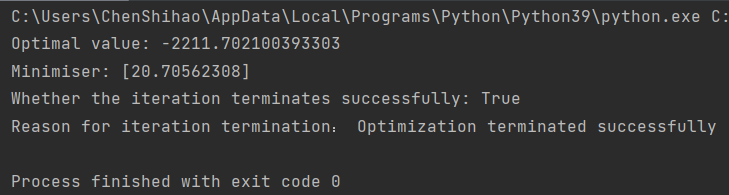
\includegraphics[width=1\textwidth]{Problem6.2.png}
    \caption{Simulation results}
    \label{f6}
    \end{figure}

% --------------------------------------------------------
% Problem 7
% --------------------------------------------------------
\section{Problem 7}

Give examples of
\subsection{}
A convex function $f:\R\rightarrow[0,\infty)$ which has a finite infimum but no minimisers.

\textbf{Solotion:}
$f(x) = \exp(x)$ whose infimum is 0, but has no minimisers.
\begin{figure}[H]
    \centering
    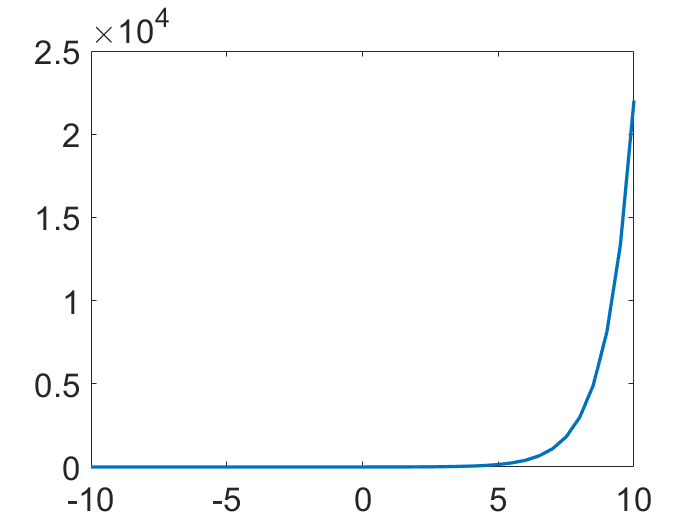
\includegraphics[height=9cm,width=16cm]{Problem7.1.png}
    \caption{$f(x) = \exp(x)$ Simulation}
    \label{f7.1}
    \end{figure}

\subsection{}
A convex function $f:\R\rightarrow\R$ that has infinitely many minimisers.

\textbf{Solotion:}
\begin{equation}
 f(x)=\left\{
\begin{array}{rcl}
-x & & {x < -2}\\
0 & & {-2 \leq x \leq 2}\\
x & & {x > 2}
\end{array} \right. 
\label{16}
\end{equation}

\begin{figure}[H]
    \centering
    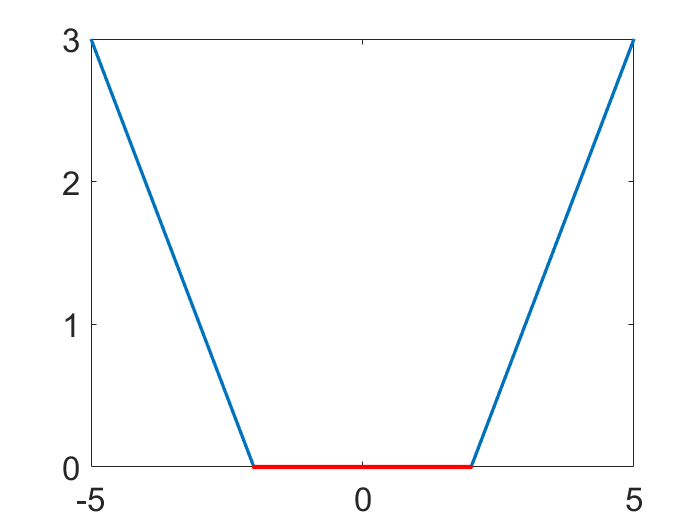
\includegraphics[height=9cm,width=16cm]{Problem7.2.png}
    \caption{$f(x)(\ref{16})$ Simulation}
    \label{f7.2}
    \end{figure}

\subsection{}
A differentiable function $f:\R\rightarrow\R$ that has a single stationary point that is not a minimiser.

\textbf{Solotion:}
$f(x) = x^3$ whose single stationary point is (0,0).
\begin{figure}[H]
    \centering
    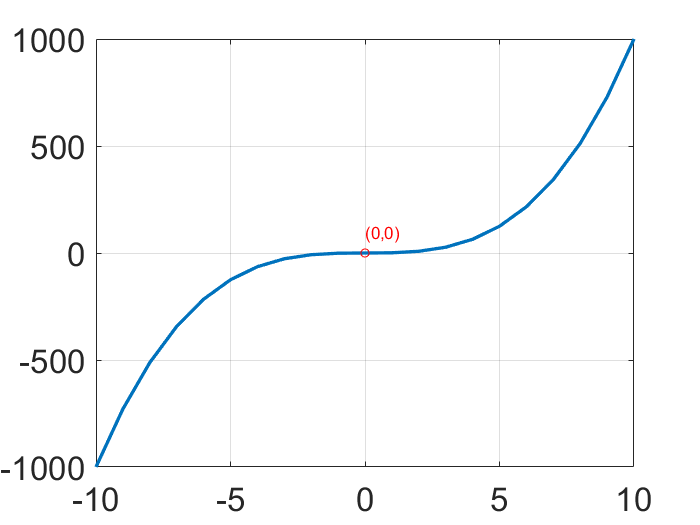
\includegraphics[height=9cm,width=16cm]{Problem7.3.png}
    \caption{$f(x) = x^3$ Simulation}
    \label{f7.3}
    \end{figure}

\subsection{}
A differentiable function $f:\R\rightarrow\R$ that has infinitely many stationary points none of which is
a minimiser.

\textbf{Solotion:}
$f(x) = x-\sin x$ whose infinitely many stationary points are in set $\{(x,y)|x=y=2k\pi,k\in \mathbb{Z}\}$.
\begin{figure}[H]
    \centering
    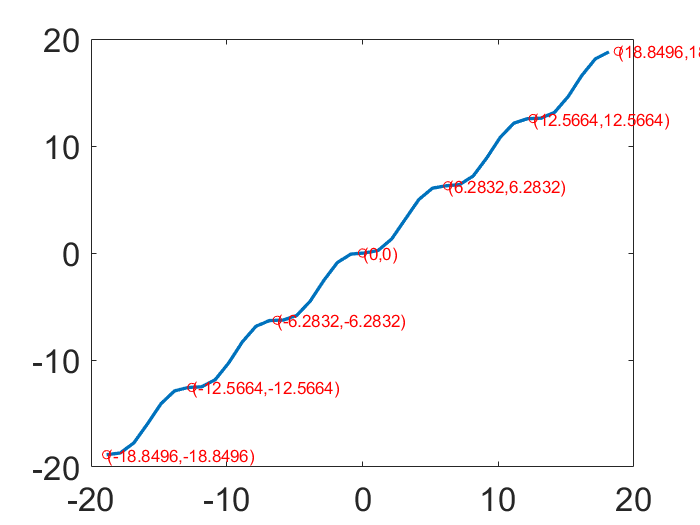
\includegraphics[height=9cm,width=16cm]{Problem7.4.png}
    \caption{$f(x) = x-\sin x$ Simulation}
    \label{f7.4}
    \end{figure}

\subsection{}
A twice differentiable function that is not constant and has infinitely many minimisers.

\textbf{Solotion:}
$f(x) = \sin(x)$ whose minimisers are in set $\{x|x=-\frac{\pi}{2}+2k\pi,k\in \mathbb{Z}\}$.
\begin{figure}[H]
    \centering
    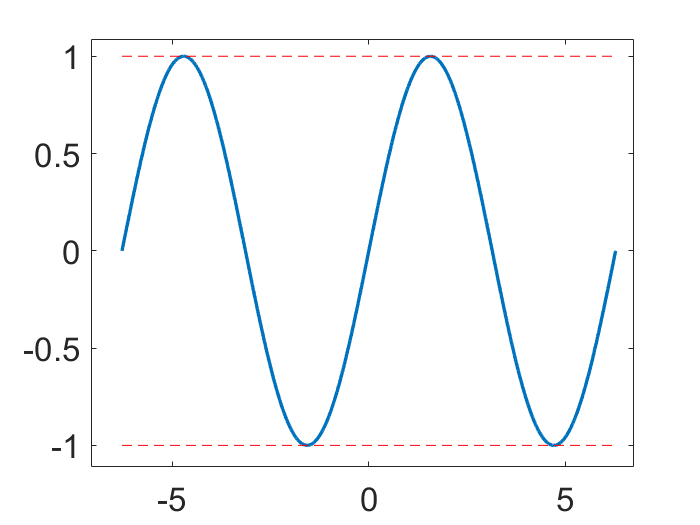
\includegraphics[height=9cm,width=16cm]{Problem7.5.png}
    \caption{$f(x) = \sin(x)$ Simulation}
    \label{f7.2}
    \end{figure}

% --------------------------------------------------------
% Problem 8
% --------------------------------------------------------
\section{Problem 8}
\subsection{}
Use the KKT theorem to solve the following problem
\begin{subequations}
    \begin{align}
        &\minimise_{\substack{x\in \R^{100}}}2\|x\|^2+3\sum_{i=1}^{50}x_i+2022,
        \\
        &\text{subject to:}\sum_{i=1}^{100}(-1)^ix_i=100.
    \end{align}
\end{subequations}
Provide a detailed derivation in your report.

\textbf{Solotion:}

The cost function is
\begin{align}
f(x)=2\|x\|^2+3\sum_{i=1}^{50} x_i+2022 \notag
\end{align}
and the  constraints are 
\begin{align}
    g(x)=\sum_{i=1}^{100}(-1)^ix_i-100 \notag
\end{align}
The Lagrangian $\mathscr{L}$ is 
\begin{align}
    \mathscr{L}(x,\lambda)&=f(x)+\lambda g(x) \notag
    \\
    &=2\|x\|^2+3\sum_{i=1}^{50} x_i+2022+\lambda(\sum_{i=1}^{100}(-1)^ix_i-100)   \notag
\end{align}
the gradient of $\mathscr{L}$ given by
\begin{align}
    \triangledown\mathscr{L}(x,\lambda)&=\begin{bmatrix} \triangledown_x\mathscr{L}(x,\lambda)  \\ \triangledown_\lambda\mathscr{L}(x,\lambda) \end{bmatrix} \notag
    \\
    &=\begin{bmatrix} 4x+b -c\lambda \\ c^{\tran}x-100 \end{bmatrix} \notag
\end{align}
where 
$$
b=
    [\underbrace {  3 \hspace{0.25em} 3 \hspace{0.25em} 3 \cdots 3}_{50} 
    \overbrace{0 \cdots 0 \hspace{0.25em} 0 \hspace{0.25em} 0  }^{50}  ]^{\tran}     
$$
$$
c=
[\underbrace {
     -1 \hspace{0.25em} 1 \hspace{0.25em} -1 \cdots 1 \hspace{0.25em} -1 \hspace{0.25em} 
    1         
} _{100} 
]
^{\tran}
$$
So that 
\begin{align}
    x^{\star}=\frac{c\lambda-b}{4}
    \label{18}
\end{align}
and 
\begin{align}
    c^{\tran}x^{\star}-100=0 \notag
    % \label{19}
\end{align}
From \ref{18}
\begin{align}
    \frac{c^{\tran}(c\lambda-b)}{4}-100=0 \notag
\end{align}
Thus
\begin{align}
    \lambda=\frac{400+c^{\tran}b}{\|c\|^{2}} \notag
\end{align}
Back to \ref{18}
\begin{align}
    x^{\star}&=\frac{c\frac{400+c^{\tran}b}{\|c\|^{2}}-b}{4} \notag
    \\
    &=\frac{c(400+c^{\tran}b)}{4\|c\|^{2}}-\frac{b}{4} \notag
\end{align}


\subsection{}

Solve the same problem using Python (e.g., CVXPy) and check whether the solution obtained
using Python is the same as the solution you obtained in Question 8.1. In your report you should
provide a link to your code and report your results.

\textbf{Solotion:}
The Python code: \href{https://github.com/Chanawesome/ELE8088-EXTRA/blob/main/Problem8.2.py}{Please Click Here}.
\begin{figure}[H]
    \centering
    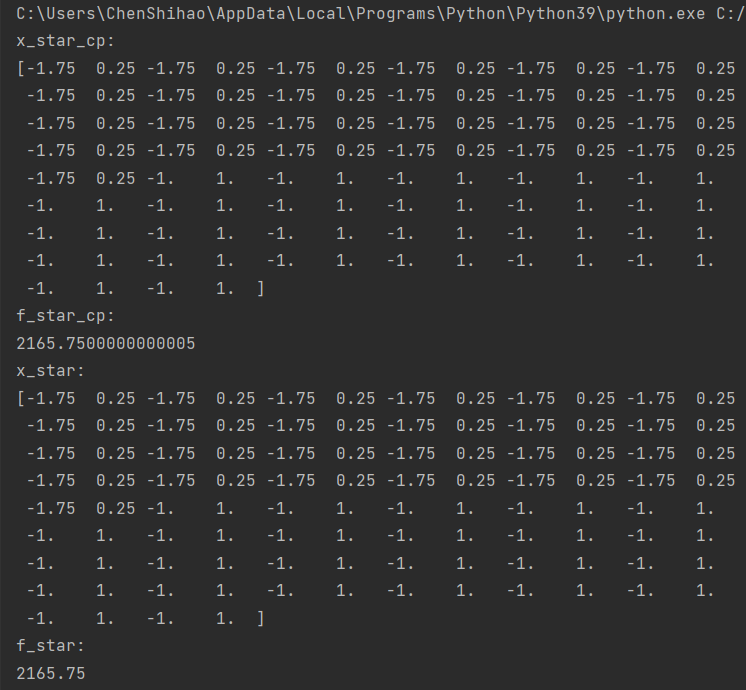
\includegraphics[width=1\textwidth]{Problem8.2.png}
    \caption{Simulation results}
    \label{f9}
\end{figure}

% --------------------------------------------------------
% Problem 10
% --------------------------------------------------------
\section{Problem 10}
\subsection{}
Give examples of discrete-time linear dynamical systems, $x_{t+1} = Ax_t + Bu_t$, with $x_t \in \R^2$ and
$u_t \in \R$, which are

1.Controllable, but not reachable

\textbf{Solotion:}

$x_{t+1}=\begin{bmatrix} 0 & 1 \\ 0 & 0 \end{bmatrix}x_t+\begin{bmatrix} 1 \\ 0 \end{bmatrix}u_t$

2.Stabilisable, but not controllable

\textbf{Solotion:}

$x_{t+1}=\begin{bmatrix} 1 & 0.5 \\ 0.5 & 1 \end{bmatrix}x_t+0\cdot u_t$

\subsection{}
Show that the following system is reachable

\begin{equation}
    x_{t+1}=\begin{bmatrix} 1 & 2 & 3 \\ 0 & 1 & -2 \\ 1 & -1 & 1 \end{bmatrix}x_t+\begin{bmatrix} 1 & 1 \\ 2 & 0 \\ 0 & 3 \end{bmatrix}u_t,
    \label{19}
\end{equation}

and determine a (finite) sequence of control actions that drives the state from the initial state x =
(0, 1, -2) to the target state x' = (2, 1, 3).

\textbf{Solotion:}

The controllability matrix,$C_3=[A^2B \hspace{0.5em} AB \hspace{0.5em} B]$,of this system \ref{19} is

$$
\begin{aligned}
    C_3=\begin{bmatrix} 6 & 10 & 5 & 10 & 1 & 1 \\ 4 & -14 & 2 & -6 & 2 & 0 \\ 2 & 20 & -1 & 4 & 0 & 3 \end{bmatrix}
\end{aligned}
$$
and the rank of $C_3$ is 3.So this system \ref{19} is reachable.
\vspace{1em}

We need to solve the equation $C_3\cdot u=x'-A^3x$,which is,
$$
\begin{aligned}
    \begin{bmatrix} 6 & 10 & 5 & 10 & 1 & 1 \\ 4 & -14 & 2 & -6 & 2 & 0 \\ 2 & 20 & -1 & 4 & 0 & 3 \end{bmatrix}
    \cdot u&=\begin{bmatrix} 2 \\ 1 \\ 3 \end{bmatrix}-\begin{bmatrix} 6 & 7 & 12 \\ -6 & 3 & -16 \\ 8 & -2 & 12 \end{bmatrix}
    \begin{bmatrix} 0 \\ 1 \\ -2 \end{bmatrix}
    \\
    \begin{bmatrix} 6 & 10 & 5 & 10 & 1 & 1 \\ 4 & -14 & 2 & -6 & 2 & 0 \\ 2 & 20 & -1 & 4 & 0 & 3 \end{bmatrix}
    \cdot u&=\begin{bmatrix} 19 \\ -34 \\ 29 \end{bmatrix}
\end{aligned}
$$
So,$u=\begin{bmatrix} -1.22185226 \\ 1.32254203 \\ -0.21643201 \\1.51523816\\-0.53635475\\-0.42817361 \end{bmatrix}$,
thus,we need to apply the control actions $u_0=\begin{bmatrix} -1.22185226 \\ 1.32254203 \end{bmatrix},
u_1=\begin{bmatrix} -0.21643201 \\1.51523816 \end{bmatrix}$ and $u_2=\begin{bmatrix} -0.53635475\\-0.42817361 \end{bmatrix}$




% Step 1:$u_1 = \begin{bmatrix} -1.72990587 \\ 1.07110789 \end{bmatrix}$,$x_1=\begin{bmatrix} -4.65879798 \\ 1.54018826 \\ 0.21332367 \end{bmatrix}$

% Step 2:$u_1 = \begin{bmatrix} -0.05677045 \\ 2.99522085 \end{bmatrix}$,$x_2=\begin{bmatrix} 1.99999995 \\ 1.00000002 \\ 2.99999998 \end{bmatrix}$

The Python code: \href{https://github.com/Chanawesome/ELE8088-EXTRA/blob/main/Problem10.2.py}{Please Click Here}.

% --------------------------------------------------------
% Problem 11
% --------------------------------------------------------
\section{Problem 11}
Consider the Riccati recursion
$$
\begin{aligned}
    P_{t+1}=Q+A^{\tran}P_tA-A^{\tran}P_tB(R+B^{\tran}P_tB)^{-1}B^{\tran}P_tA,
\end{aligned}
$$

where

$$
\begin{aligned}
    A = \begin{bmatrix} 2 & 1 \\ 1 & 0 \end{bmatrix},
\end{aligned}
$$
$$
\begin{aligned}
    B = \begin{bmatrix} 2 \\ -1 \end{bmatrix},
\end{aligned}
$$
$$
\begin{aligned}
    Q = \begin{bmatrix} 1 & 1 \\ 1 & 1 \end{bmatrix},
\end{aligned}
$$
$$
\begin{aligned}
    R = 2,
\end{aligned}
$$
$$
\begin{aligned}
    P_0 = \begin{bmatrix} 2 & 0 \\ 0 & 0 \end{bmatrix},
\end{aligned}
$$

\subsection{}
Is it true that this Riccati recursion converges? Justify your answer and check all conditions
carefully. As a hint, note that $Q$ can be written as $Q = qq^{\tran}$ with $q =\begin{bmatrix} 1 \\ 1 \end{bmatrix}$. 

\textbf{Solotion:}

The controllability matrix,$C_2$ of $(A,B)$ is,

$$
\begin{aligned}
    C_2=[AB \hspace{0.5em} B]=\begin{bmatrix} 3 & 2 \\ 2 & -1 \end{bmatrix}
\end{aligned}
$$
The rank of $C_2$ is 2,so $(A,B)$ is controllable.

Since $Q = q^{\tran}q$ with $q =\begin{bmatrix} 1 & 1 \end{bmatrix}$. 
$$
\begin{aligned}
    \mathcal{O}&=\begin{bmatrix} q \\ qA \end{bmatrix}
    \\
    &=\begin{bmatrix} 1 & 1 \\ 3 & 1 \end{bmatrix}
\end{aligned}
$$
The rank of $\mathcal{O}$ is 2,so $(A,q)$ is observable.

And $Q\in\mathbb{S}_+,R\in\mathbb{S}_{++},P_0\in\mathbb{S}_+$

So $P=\lim_{t\rightarrow\infty}P_t$ exists which means this Riccati recursion converges.

\subsection{}
Use control.dare in Python to determine the limit $\lim_{t\rightarrow\infty} P_t$. Include this limit in your report
and provide a link to your code.

\textbf{Solotion:}
The Python code: \href{https://github.com/Chanawesome/ELE8088-EXTRA/blob/main/Problem11.2.py}{Please Click Here}.
\begin{figure}[H]
    \centering
    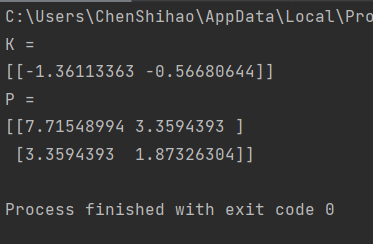
\includegraphics[height=9cm,width=16cm]{Problem11.2.png}
    \caption{Simulation results}
    % \label{f9}
\end{figure}

% --------------------------------------------------------
% Problem 14
% --------------------------------------------------------
\section{Problem 14}
Let $X$ be a continuous random variable with pdf
$$ p_X(x)=\left\{
\begin{aligned}
\frac{2}{x^2}&,\text{for} \hspace{0.3em} x \in [1,2), \\
0&,   \text{otherwise} 
\end{aligned}
\right.
$$
\subsection{}
Determine P$[X \geq$ 1.5]

\textbf{Solotion:}
$$
\begin{aligned}
P[X \geq 1.5]&=\int_{1.5}^{\infty} p_X(x) dx
\\
&=\int_{1.5}^{2} \frac{2}{x^2} dx + \int_{2}^{\infty} 0 dx
\\
&=\int_{1.5}^{2} \frac{2}{x^2} dx
\\
&=-\frac{2}{x}\bigg|_{1.5}^2
\\
&=\frac{1}{3}
\end{aligned}
$$

\subsection{}
Determine $\mathbb{E}[X]$ and Var$[X]$

\textbf{Solotion:}
$$
\begin{aligned}
    \mathbb{E}[X]&=\int_{-\infty}^{\infty} xp_X(x) dx
    \\
    &=\int_{1}^{2} \frac{2}{x^2} dx
    \\
    &=-\frac{2}{x}\bigg|_{1}^2
    \\
    &=1
\end{aligned}
$$
\vspace{1em}
$$
\begin{aligned}
    \text{Var}[X]&=\mathbb{E}[(X-\mathbb{E}[X^2])^2]
    \\
    &=\int_{-\infty}^{\infty} (x-\mathbb{E}[X])^2p_X(x) dx
    \\
    &=\int_{1}^{2} (x-1)^2\frac{2}{x^2} dx
    \\
    &=\int_{1}^{2} \frac{2x^2-4x+2}{x^2} dx
    \\
    &=\int_{1}^{2} 2-\frac{4}{x}+\frac{2}{x^2} dx
    \\
    &=-4\ln x\bigg|^2_1+\frac{-2}{x}\bigg|^2_1
    \\
    &=-4\ln2+1
\end{aligned}
$$


\subsection{}
Determine $\mathbb{E}[X^3]$ using the law of the unconscious statistician

\textbf{Solotion:}

$$
\begin{aligned}
    \mathbb{E}[X^3]&=\int_{-\infty}^{\infty}x^3p_X(x) dx
    \\
    &=\int_{1}^{2}x^3\frac{2}{x^2} dx
    \\
    &=x^2\bigg|^2_1
    \\
    &=3
\end{aligned}
$$

% --------------------------------------------------------
% Problem 16
% --------------------------------------------------------
\section{Problem 16}
Alice has two coins in her pocket, a fair coin (heads on one side and tails on the other side) and a
two-headed coin (heads on both sides). She picks one at random from her pocket, tosses it and obtains
heads. What is the probability that she flipped the fair coin?

\textbf{Solotion:}

P[fair coin]=P[two-headed coin]=50\%,,P[heads$|${fair coin}]=50\%,P[heads$|${two-headed coin}]=1,such that
$$
\begin{aligned}
    \text{P[heads}]&=\text{P[heads}|{\text{fair coin}}]\cdot \text{P[fair coin}]+
    \\
    &\text{P[heads}|{\text{two-headed coin}}]\cdot \text{P[two-headed coin}]
    \\
    &=50\%\cdot 50\%+1\cdot 50\%
    \\
    &=75\%
\end{aligned}
$$
\vspace{1em}
$$
\begin{aligned}
    \text{P[fair coin}| \text{heads}]&=\frac{\text{P[heads}| \text{fair coin}]\cdot\text{P[fair coin}]}{\text{P[heads}]}
    \\
    &=\frac{50\%\cdot 50\%}{75\%}
    \\
    &=\frac{1}{3}
\end{aligned}
$$

% --------------------------------------------------------
% Problem 17
% --------------------------------------------------------
\section{Problem 17}
You have a coin that has probability $p$ of landing heads and probability 1 - $p$ of landing tails. You
believe that the coin is fair. To that end, you treat $p$ as a random variable with expectation 
$\mathbb{E}[p]$ = 0.5
and variance Var[$p$] = 0.0119; you may choose any appropriate prior distribution for $p$ that has such
an expectation and variance.

You flip the coin 25 times and you obtain the following observations:

\vspace{1em}

Heads, Heads, Heads, Tails, Heads, Heads, Tails, Heads, Heads, Heads, Heads, Tails, Heads, Heads,
Tails, Tails, Heads, Heads, Tails, Tails, Heads, Heads, Heads, Heads, Heads.(18H,7T)

\subsection{}
What is the posterior distribution of $p$ given these measurements? Include a plot in your report.

\textbf{Solotion:}

% $$
% \begin{aligned}
%     L(p|25,x)=\bigg(\frac{25!}{x!(25-x)!}\bigg)p^x(1-p)^{25-x}
% \end{aligned}
% $$

% $$
% \begin{aligned}
%     \ln L(p|25,x)&=\ln\bigg[\bigg(\frac{25!}{x!(25-x)!} \bigg)p^x(1-p)^{25-x}  \bigg]
%     \\
%     &=\ln\bigg(\frac{25!}{x!(25-x)!}\bigg)+\ln(p^x)+\ln[(1-p)^{25-x}]
%     \\
%     &=\ln\bigg(\frac{25!}{x!(25-x)!}\bigg)+x\ln(p)+(25-x)\ln(1-p)
% \end{aligned}
% $$


% \begin{equation}
%     \frac{d \ln L(p|25,x)}{dp}=0+x\frac{1}{p}+x\frac{1}{1-p}-25\frac{1}{1-p}
%     \label{20}
% \end{equation}
% Let equation \ref{20} equals to 0,
% $$
% \begin{aligned}
%     \frac{d \ln L(p|25,x)}{dp}=x\frac{1}{p}+x\frac{1}{1-p}-25\frac{1}{1-p}=0
% \end{aligned}
% $$
% Thus,
% $$
% \begin{aligned}
%     x(1-p)+xp-25p=0
% \end{aligned}
% $$
% Which is,
% $$
% \begin{aligned}
%     x-25p=0
% \end{aligned}
% $$
% So,
% $$
% \begin{aligned}
%     p=\frac{x}{25}
% \end{aligned}
% $$
We have,
$$
\begin{aligned}
    \mathbb{E}[p]&=\frac{\alpha}{\alpha+\beta}=0.5  
    \\
    \text{Var}[p]&=\frac{\alpha\beta}{(\alpha+\beta+1)(\alpha+\beta)^2}=0.0119
\end{aligned}
$$
Thus,
$$
\begin{aligned}
    \alpha=\beta=10
\end{aligned}
$$
The posterior distribution is,
$$
\begin{aligned}
    p|x_1,x_2,x_3,\dots,x_{25} &\sim \text{Beta}(\sum_{i=1}^{10}x_i+\alpha,25-\sum_{i=1}^{10}x_i+\beta) 
    \\
    &=\text{Beta}(18+10,25-18+10)
    \\
    &=\text{Beta}(28,17)
\end{aligned}
$$

\begin{figure}[H]
    \centering
    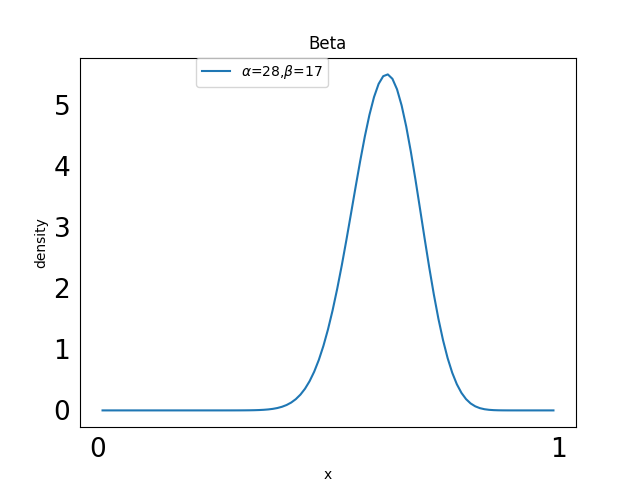
\includegraphics[width=1\textwidth]{Problem17.1.png}
    \caption{Beta Distribution}
    \label{f17.1}
    \end{figure}

% It is clear,
% $$
% \begin{aligned}
%     \theta|x \sim Beta(x+1,26-x)
% \end{aligned}
% $$
% Which is,
% $$
% \begin{aligned}
%     \theta|x \sim Beta(19,8)
% \end{aligned}
% $$
\subsection{}
What is the maximum a posteriori (MAP) estimate of $p$ given these measurements?

\textbf{Solotion:}

$$
\begin{aligned}
    \hat{\theta}_{MAP}=\frac{28-1}{28+17-2}=\frac{27}{43}
\end{aligned}
$$

\subsection{}
What is the posterior mean given these measurements?

\textbf{Solotion:}





% --------------------------------------------------------
% Problem 18
% --------------------------------------------------------
\section{Problem 18}
Let N be the number of customers that enter a store in a given day and we know that $\mathbb{E}[N]$ = 20
and Var[$N$] = 25. Let $X_i$ be the amount of money that the $i$-th customer spends and assume that
the $X_i$ are independent random variables and independent of $N$.
Assume that $\mathbb{E}[X_i]$ = £20 and Var[$X_i$] = \pounds100 for all $i$ = 1,..., $N$. 
The Y be the store's total sales,
$$
\begin{aligned}
    Y=\sum^N_{i=1}X_i.
\end{aligned}
$$

\subsection{}
Determine $\mathbb{E}[Y]$ using the law of total expectation

\textbf{Solotion:}

$$
\begin{aligned}
    \mathbb{E}[Y]&=\mathbb{E}[\mathbb{E}[Y|N]]=\mathbb{E}[\mathbb{E}[\sum^N_{i=1}X_i|N]]
    \\
    &=\mathbb{E}[\sum^N_{i=1}\mathbb{E}[X_i|N]]
    \\
    &=\mathbb{E}[20N]=20\mathbb{E}[N]
    \\
    &=400
\end{aligned}
$$

\subsection{}
Determine Var[$Y$] using the law of total variance

\textbf{Solotion:}

$$
\begin{aligned}
    \text{Var}[\mathbb{E}[Y|N]]=\text{Var}[20N]=400\cdot 25=10000
\end{aligned}
$$
\vspace{1em}
$$
\begin{aligned}
    \text{Var}[Y|N]&=\text{Var}[[\sum^N_{i=1}X_i|N]]
    \\
    &=\sum^N_{i=1}\text{Var}[X_i|N]
    \\
    &=100N
\end{aligned}
$$
\vspace{1em}
$$
\begin{aligned}
    \text{Var}[Y]&=\mathbb{E}[\text{Var}[Y|N]]+\text{Var}[\mathbb{E}[Y|N]]
    \\
    &=\mathbb{E}[100N]+10000
    \\
    &=100\cdot 20+10000
    \\
    &=12000
\end{aligned}
$$

% --------------------------------------------------------
% Problem 25
% --------------------------------------------------------
\section{Problem 25}
Describe the extended Kalman filter and the moving horizon estimation methodologies (you are ex-
pected to provide technical details). What are the merits and limitations of each approach?

\textbf{Solotion:}

$^{\star}$Extended Kalman Filter:

Extended Kalman filtering can be used to solve problems in nonlinear cases by Taylor expansion.
Obviously, the tangent at the point with the largest possible value in the original distribution 
should be used, which is the tangent at the mean, as shown in \ref{f12}. The result 
(dashed line) is closer to the mean variance of the actual result.%(MERITS)

\begin{figure}[H]
    \centering
    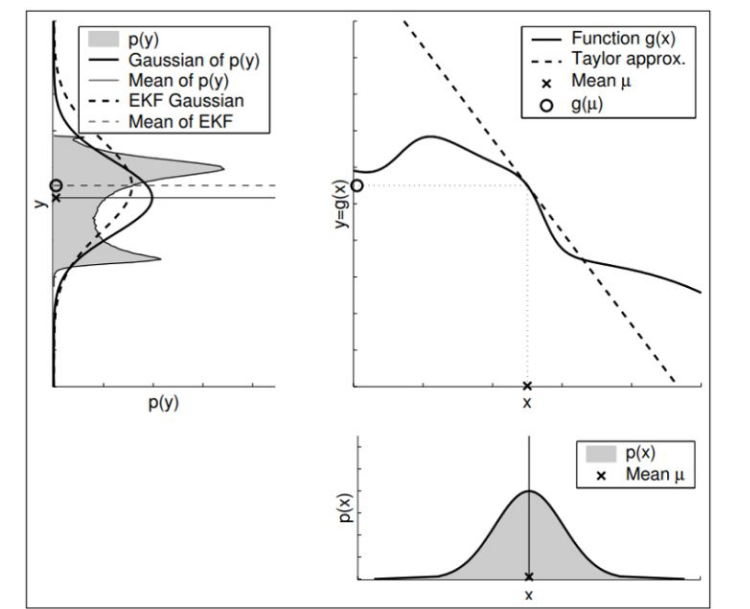
\includegraphics[width=1\textwidth]{Problem25.png}
    \caption{Extended Kalman Filter}
    \label{f12}
    \end{figure}

For EKF,linearize at a time when the nearest state $x_{k-1}$ , the nearest input $u_{k-1}$ , 
and 0 noise are known,

Equation of motion,
$$
\begin{aligned}
    x_k=f_{k-1}(x_{k-1},u_{k-1},w_{k-1}) \approx f_{k-1}(\hat{x}_{k-1},u_{k-1},0)
    \\
    +\frac{\partial f_{k-1}}{\partial x_{k-1}}|_{\hat{x}_{k-1},u_{k-1},0}(x_{k-1}-\hat{x}_{k-1})
    +\frac{\partial f_{k-1}}{\partial w_{k-1}}|_{\hat{x}_{k-1},u_{k-1},0}w_{k-1}
\end{aligned}
$$

Observation equation,
$$
\begin{aligned}
    y_k=h_k(x_k,v_k) \approx h_k(\hat{x}_k,0)+\frac{\partial h_{k}}{\partial x_{k}}|_{\hat{x}_k,0}
    (x_k-\hat{x}_k)+\frac{\partial h_{k}}{\partial v_{k}}|_{\hat{x}_k,0}v_k
\end{aligned}
$$

The four Jocabian matrices are as follows,
$$
\begin{aligned}
    &F_{k-1}=\frac{\partial f_{k-1}}{\partial x_{k-1}}|_{\hat{x}_{k-1},u_{k-1},0}
    \\
    &L_{k-1}=\frac{\partial f_{k-1}}{\partial w_{k-1}}|_{\hat{x}_{k-1},u_{k-1},0}
    \\
    &H_k=\frac{\partial h_{k}}{\partial x_{k}}|_{\hat{x}_k,0}
    \\
    &M_k=\frac{\partial h_{k}}{\partial v_{k}}|_{\hat{x}_k,0}
\end{aligned}
$$

Linearized motion model,
$$
\begin{aligned}
    x_k=f_{k-1}(\hat{x}_{k-1},u_{k-1},0)+F_{k-1}(x_{k-1}-\hat{x}_{k-1})+L_{k-1}w_{k-1}
\end{aligned}
$$

Linearized measurement model,
$$
\begin{aligned}
    y_k=h_k(\hat{x}_k,0)+H_k(x_k-\hat{x}_k)+M_kv_k
\end{aligned}
$$

Prediction,
$$
\begin{aligned}
    &\hat{x}_k=f_{k-1}(\hat{x}_{k-1},u_{k-1},0)
    \\
    &\hat{P}_k=F_{k-1}\hat{P}_{k-1}F^{\tran}_{k-1}+L_{k-1}Q_{k-1}L^{\tran}_{k-1}
\end{aligned}
$$

Optimal gain,
$$
\begin{aligned}
    K_k=\hat{P}_kH^{\tran}_{k}(H_k\hat{P}_kH^{\tran}_{k}+M_kR_kM^{\tran}_{k})^{-1}
\end{aligned}
$$

Correction,

$$
\begin{aligned}
    &\hat{x}_k=\hat{x}_k+K_k(y_k-h_k(\hat{x}_k,0))
    \\
    &\hat{P}_k=(1-K_kF_k)\hat{P}_k
\end{aligned}
$$

Linearization is performed by computing a local linear approximation of the nonlinear function with respect to the selected operating point.
Linearization relies on computing the Jacobian matrix (consisting of the first partial derivatives of the function)

From the main idea of EKF, it is not difficult to see that since only the first-order 
approximation is used, in subsequent iterations, the error may become larger and larger. 
This is also its disadvantage.

\vspace{2em}

$^{\star}$Moving Horizon Estimation:

Moving horizon estimation is an optimization-based state-estimation technique where the 
current state of the system is inferred based on a finite sequence of past measurements.

In comparison to more traditional state-estimation methods, e.g. the extended Kalman filter (EKF), 
MHE will often outperform the former in terms of estimation accuracy. 
This is especially true for non-linear dynamical systems, 
which are treated rigorously in MHE and where the EKF is known to work reliably only if the 
system is almost linear during updates.

Another advantage of MHE is the possible incorporation of further constraints on estimated 
variables. These can be used to enforce physical bounds, e.g. fractions between 0 and 1.

All of this comes at the cost of additional computational complexity.

The basic idea of MHE is to estimate the state trajectory using only the past N measurements, 
where N is referred to the length of horizon window. An nonlinear programming (NLP) problem is 
formulated at each sample time where a batch of past measurements is introduced and the states 
are estimated simultaneously. The horizon window allows incorporation of both frequent and 
infrequent measurements where the slow ones can be introduced as they are available.

The MHE formulation is shown as,
\begin{subequations}
    \begin{align}
    &\min_{\substack{z_l-N}}n\|z_l-N-  \overline{z}_l-N\|^2W_z+\sum^N_{l=0}\|y_l- \overline{y}_{l+k-N}\|^2W_y
    \label{20a}
    \\
    &\text{s.t.}z_{l+1}=f(z_l,u_l)+w_l
    \label{20b}
    \\
    &y_l=h(z_l)+v_l
    \label{20c}
    \end{align}
\end{subequations}

% \ref{20a}\ref{20b}\ref{20c}
where the process is assumed to be modelled by Eq. \ref{20b} \ref{20c},$z_l$  is the vector of states,
$u_l$ is the vector of inputs,$y_l$ is the vector of measurements,$w_l$is the vector of unknown disturbances, and
$v_l$  is the vector of measurement noise. The noise variables are assumed to be independent of states and 
$w_l \sim N(0,Q_l)$ and $v_l \sim N(0,R_l)$.$W_z,W_y$ represent the inverse of the covariance matrices of the prior state estimates
$\overline{z}_{l-N}$ and measurement $\overline{y}_{l+k-N}$, respectively.The state vector is denoted as  
$z_l=[x_l,p_l]$,where$x_l$ are  the reactant concentrations, and $p_l$ are kinetic parameters and
$r_a(j)$.It is also assumed the bounds and constraints of states can be further added in the NLP formulation.

% --------------------------------------------------------
% Problem 22
% --------------------------------------------------------
\section{Problem 22}
Consider the system
$$
\begin{aligned}
    &x_{t+1}=Ax_t+Bu_t+Gw_t,
    \\
    &y_t=Cx_t+v_t,
\end{aligned}
$$
where (i) $x_0$ is a random variable and (iv) $x_0 \sim \mathcal{N}(\widetilde{x}_0,P_0)$,
(ii) $\mathbb{E}[w_t]=0$ and $\mathbb{E}[v_t]=0$ for all $t\in\N$,(iii) $x_0,(w_t)_t$ and $(v_t)_t$
are mutually independent random variables, (iii) $w_t$ and $v_t$  are normallydistributed and 
$\mathbb{E}[w_tw_t^{\tran}]=Q,\mathbb{E}[v_tv_t^{\tran}]=R$.Determine the covariance matrix
$P_{t,l}=$Cov$(x_t,x_l)$ for $t,l\in\N$,as a function of $P_0,A,G,Q,t$ and $l$.

\textbf{Solotion:}

Assume $l\geq t$.If $l=t$, 
$$
\begin{aligned}
    P_{t,t}=\text{Cov}(x_t,x_t)=\text{Var}(x_t) 
\end{aligned}
$$
We have,
\begin{subequations}
    \begin{align}
    &P_{0,0}=P_0 
    \\
    &P_{t+1}=AP_tA^{\tran}+Q
\end{align}
\end{subequations}
If $l=t+1$,
$$
\begin{aligned}
    \text{Cov}(x_t,x_{t+1})&=\text{Cov}(x_t,Ax_t+Bu_t+Gw_t)
    \\
    &=\text{Cov}(x_t,Ax_t)+\text{Cov}(x_t,Bu_t)+\text{Cov}(x_t,Gw_t)
    \\
    &=\text{Cov}(x_t,x_t)\cdot A^{\tran}+\text{Cov}(x_t,x_t)\cdot B^{\tran}+\text{Cov}(x_t,x_t)\cdot G^{\tran}
    \\
    &=P_t\cdot A^{\tran}+P_t\cdot B^{\tran}+P_t\cdot G^{\tran}
\end{aligned}
$$
And,
\begin{subequations}
    \begin{align}
    \text{Cov}(x_t,x_{t+2})&=P_t\cdot (A^{\tran})^2+P_t\cdot (B^{\tran})^2+P_t\cdot (G^{\tran})^2
    \\
    \text{Cov}(x_t,x_{t+3})&=P_t\cdot (A^{\tran})^3+P_t\cdot (B^{\tran})^3+P_t\cdot (G^{\tran})^3
    \\
    \vdots \notag
    \\
    \text{Cov}(x_t,x_{t+n})&=P_t\cdot (A^{\tran})^n+P_t\cdot (B^{\tran})^n+P_t\cdot (G^{\tran})^n
    \label{22c}
\end{align}
\end{subequations}
Where,
\begin{subequations}
    \begin{align}
    P_1&=AP_0A^{\tran}+Q
    \\
    P_2&=AP_1A^{\tran}+Q=A(AP_0A^{\tran}+Q)A^{\tran}+Q=A^2P_0(A^{\tran})^2+AQA^{\tran}+Q
    \\
    P_3&=A^3P_0(A^{\tran})^3+A^2Q(A^{\tran})^2+AQA^{\tran}+Q
    \\
    \vdots \notag
    \\
    P_t&=A^tP_0(A^{\tran})^t+A^{t-1}Q(A^{\tran})^{t-1}+A^{t-2}Q(A^{\tran})^{t-2}+\cdots+A^{t-t}Q(A^{\tran})^{t-t}+Q
    \label{23d}
\end{align}
\end{subequations}

Combining with \ref{22c} and \ref{23d},
$$
\begin{aligned}
    \text{Cov}(x_t,x_l)=
\end{aligned}
$$








% \clearpage
% \begin{tcolorbox}[title={Common typesetting mistakes}]
%     \textbf{Important Note:}
%     Write $\cos x$, not $cos x$.
%     Write $\sin x$, $\log x$, etc --- not $sin x$, $log x$ and so on.
%     Write $\lim_{s\to 0^+} sF(s)$, not $lim_{s\to 0^+} sF(s)$.
%     Write $xy$,  or $x\cdot y$,  but never $x*y$ --- that would be the \textit{convolution} of $x$ with $y$,  not their product,  so
%     \begin{equation}
%         2 * 3 = 3t^2.
%     \end{equation}
%     To denote a variable with a subscript, write $x_1$, not $x1$.
%     For superscripts, write $x^2$, not $x2$.
%     Denote a variable by $x$, not x.
%     Write $x_t$, not x$_t$.
%     Double quotes are ``like this'',  not "like this".
%     Reference equations using: Equation \eqref{eq:partial_derivatives};
%     not Equation \ref{eq:partial_derivatives} and not Equation (12).
% \end{tcolorbox}

% \begin{tcolorbox}[title={Additional typesetting mistakes}]
%     A few more things to keep in mind:
%     \begin{enumerate}
%         \item The set of real numbers is denoted as $\R$, not $R$
%         \item The set of symmetric positive (semi)definite matrices of dimensions $n$-by-$n$ is denoted as ($\Sp^n$) $\Spp^n$.
%         \item Alternatively we can write ($A \succcurlyeq 0$) $A \succ 0$.
%         \item The expectation of $X$ is $\E[X]$ (not $E[X]$, not $IE[X]$). Its variance is $\Var[X]$.
%         \item Cost functions are $\ell(x, u)$, not $l(x, u)$
%         \item The norm of $x$ is $\|x\|$, not $||x||$
%         \item The ball of radius $\eta>0$ is $\mathcal{B}_\eta$
%         \item Denote the conditional expectation of $X$ given $Y$ like this: $\E[X {}\mid{} Y]$
%         \item Probabilities are denoted as $\prob[X \in A]$.
%         \item The mass of an object can be $\unit[1]{kg}$, not $1kg$ and not $1$ kg.
%         \item The ``greater than or equal'' symbol is $\geq$, not $>=$
%         \item Minimisers are denoted with $x^\star$, not $x^*$
%         \item $\sum$ (sum) is not the same as $\Sigma$ (sigma uppercase)
%     \end{enumerate}
% \end{tcolorbox}

% \vspace{1em}
% \begin{tcolorbox}[title={Language and style}]
%     Please keep in mind:
%     \begin{enumerate}
%         \item Use formal language and avoid contractions (isn't,  doesn't, etc)
%         \item Use impersonal language. Do not write: ``As you can see here...'' Write: ``It can be seen that...''
%         \item Do not ever use the pronoun ``I.''
%         \item The symbols $=$, $\exists$, $\forall$ are mathematical symbols. You should not write ``the state of the system at time $0$ is $=x$.'' Instead write ``the state at time $t=0$ is $x$,'' or ``$x_0 = x$''. Likewise, do not write ``the probability that a person is $>\unit[60]{kg}$ is $\leq 0.8$.'' Instead, write ``the probability that a person's weight is higher than $\unit[60]{kg}$ does not exceed $0.8$.''
%         \item Use ``$\Rightarrow$'' and ``$\Leftrightarrow$'' in equations and mathematical expressions; use the words ``therefore, so, (thus, hence)'' in your discussion.
%         \item Punctuate your equations (as in this document).
%     \end{enumerate}
% \end{tcolorbox}





\end{document}
